\chapter{Camadas eletrônicas e tabela periódica}\label{ch:g10:electron-shells}

O neônio brilha em vermelho-alaranjado num letreiro; o sódio, um \omterm{def:g9:periodic-table-first-look:metal}{metal}
mole, pega fogo na água; o cloro é um gás amarelo-esverdeado sufocante.
No entanto, os \omterm{def:g7:atoms-and-molecules:atom}{átomos} deles diferem por apenas um ou dois \omterm{def:g9:inside-the-atom:proton}{prótons}: o
neônio tem 10, o sódio 11, o cloro 17. Por que vizinhos na \omterm{def:g9:periodic-table-first-look:periodic-table}{tabela
periódica} se comportam de modo tão diferente, enquanto o sódio e o
potássio, distantes em \omterm{def:g9:inside-the-atom:atomic-number}{número atômico}, se comportam de modo tão
parecido? A resposta está no modo como os \omterm{def:g9:inside-the-atom:nucleus}{elétrons} de um \omterm{def:g7:atoms-and-molecules:atom}{átomo} estão
organizados.

\begin{recall}
Um \omterm{def:g7:atoms-and-molecules:atom}{átomo} tem $Z$ \omterm{def:g9:inside-the-atom:proton}{prótons} no \omterm{def:g9:inside-the-atom:nucleus}{núcleo} e, quando neutro, $Z$ \omterm{def:g9:inside-the-atom:nucleus}{elétrons} em
volta dele (\cref{ch:g9:inside-the-atom}). A \omterm{def:g9:periodic-table-first-look:periodic-table}{tabela periódica} ordena os
elementos por $Z$ em períodos (linhas) e grupos (colunas); os elementos
de um grupo se comportam de modo parecido
(\cref{ch:g9:periodic-table-first-look}). Os \omterm{def:g7:atoms-and-molecules:atom}{átomos} ganham ou perdem
\omterm{def:g9:inside-the-atom:nucleus}{elétrons} e viram \omterm{def:g9:ions:ion}{íons} (\cref{ch:g9:ions}).
\end{recall}

\section{A configuração eletrônica}

\begin{definition}[Camadas, subníveis e configuração eletrônica]\label{def:g10:electron-shells:configuration}
Os \omterm{def:g9:inside-the-atom:nucleus}{elétrons} de um \omterm{def:g7:atoms-and-molecules:atom}{átomo} estão organizados em
\emph{camadas}\index{camada}, numeradas $n = 1, 2, 3, \ldots$ do \omterm{def:g9:inside-the-atom:nucleus}{núcleo}
para fora; quanto maior $n$, mais longe do \omterm{def:g9:inside-the-atom:nucleus}{núcleo} e menos presos estão
os \omterm{def:g9:inside-the-atom:nucleus}{elétrons}. Cada camada se divide em
\emph{subníveis}\index{subnivel@subnível}, designados por uma letra: a camada 1
tem um subnível s (1s), a camada 2 um subnível s e um p (2s, 2p), a
camada 3 tem 3s e 3p (e 3d, visto mais tarde). Um subnível s comporta no
máximo 2 \omterm{def:g9:inside-the-atom:nucleus}{elétrons}, um subnível p no máximo 6. A \emph{configuração
eletrônica}\index{configuracao eletronica@configuração eletrônica} de um \omterm{def:g7:atoms-and-molecules:atom}{átomo} lista os seus
subníveis ocupados, com os seus números de \omterm{def:g9:inside-the-atom:nucleus}{elétrons} como expoentes:
$1\mathrm{s}^2\,2\mathrm{s}^2\,2\mathrm{p}^4$ para o oxigênio.
\end{definition}

\begin{method}[Escrever uma configuração eletrônica, até $Z = 20$]\label{met:g10:electron-shells:write}
\begin{enumerate}
  \item Conte os \omterm{def:g9:inside-the-atom:nucleus}{elétrons}: $Z$ para um \omterm{def:g7:atoms-and-molecules:atom}{átomo} neutro.
  \item Preencha os \omterm{def:g10:electron-shells:configuration}{subníveis} nesta ordem, cada um até o seu máximo
        antes de começar o seguinte:
        \[
          1\mathrm{s} \to 2\mathrm{s} \to 2\mathrm{p} \to 3\mathrm{s} \to
          3\mathrm{p} \to 4\mathrm{s}.
        \]
  \item Verifique que os expoentes somam o número de \omterm{def:g9:inside-the-atom:nucleus}{elétrons}.
\end{enumerate}
Sódio, $Z = 11$: $1\mathrm{s}^2\,2\mathrm{s}^2\,2\mathrm{p}^6\,3\mathrm{s}^1$.
Cloro, $Z = 17$: $1\mathrm{s}^2\,2\mathrm{s}^2\,2\mathrm{p}^6\,3\mathrm{s}^2\,3\mathrm{p}^5$.
Cálcio, $Z = 20$: $1\mathrm{s}^2\,2\mathrm{s}^2\,2\mathrm{p}^6\,3\mathrm{s}^2\,3\mathrm{p}^6\,4\mathrm{s}^2$.
\end{method}

\begin{omfigure}
\begin{tikzpicture}[font=\small, y=0.95cm]
  \draw[->, black!60] (-0.4,0) -- (-0.4,5.4) node[above, align=center, font=\footnotesize]
    {mais longe\\ do núcleo};
  \foreach \y/\lab/\n/\x in {0.3/1s/2/0.5, 1.3/2s/2/0.5, 1.9/2p/6/2.4, 3.0/3s/2/0.5,
      3.6/3p/6/2.4, 4.4/4s/2/0.5} {
    \foreach \k in {1,...,\n} \draw[omDef, fill=omDef!10] (\x+0.42*\k-0.42,\y) rectangle ++(0.36,0.36);
    \node[anchor=east] at (\x-0.05,\y+0.18) {\lab};
  }
  \node[anchor=west, font=\footnotesize] at (5.3,0.48) {camada 1: 2 elétrons no máximo};
  \node[anchor=west, font=\footnotesize] at (5.3,1.7) {camada 2: $2 + 6 = 8$};
  \node[anchor=west, font=\footnotesize] at (5.3,3.4) {camada 3: $2 + 6 = 8$ (até $Z = 18$)};
  \node[anchor=west, font=\footnotesize] at (5.3,4.58) {4s se preenche antes de 3d};
\end{tikzpicture}

{\small A ordem de preenchimento, até $Z = 20$. Cada caixinha é um lugar
para um \omterm{def:g9:inside-the-atom:nucleus}{elétron}: um \omterm{def:g10:electron-shells:configuration}{subnível} s tem 2 lugares, um \omterm{def:g10:electron-shells:configuration}{subnível} p tem 6.}
\end{omfigure}

\section{Os elétrons de valência}

\begin{definition}[Elétrons de valência e elétrons internos]\label{def:g10:electron-shells:valence}
Os \omterm{def:g9:inside-the-atom:nucleus}{elétrons} da \omterm{def:g10:electron-shells:configuration}{camada} ocupada mais externa (a camada de maior $n$) são
os \emph{elétrons de valência}\index{eletron de valencia@elétron de valência}; os outros são
os \emph{elétrons internos}\index{eletron interno@elétron interno}. Só os \omterm{def:g9:inside-the-atom:nucleus}{elétrons} de
valência participam das \omterm{def:g7:chemical-reactions:reaction}{reações químicas}.
\end{definition}

\begin{example}[Contar os elétrons de valência]\label{ex:g10:electron-shells:count}
Oxigênio, $1\mathrm{s}^2\,2\mathrm{s}^2\,2\mathrm{p}^4$: \omterm{def:g10:electron-shells:configuration}{camada} externa $n =
2$, $2 + 4 = 6$ \omterm{def:g10:electron-shells:valence}{elétrons de valência}. Sódio, $\ldots 3\mathrm{s}^1$: 1
\omterm{def:g10:electron-shells:valence}{elétron de valência}. Cloro, $\ldots 3\mathrm{s}^2\,3\mathrm{p}^5$: 7.
Neônio, $1\mathrm{s}^2\,2\mathrm{s}^2\,2\mathrm{p}^6$: 8, uma camada
completa.
\end{example}

\section{A tabela reconstruída a partir das configurações}

\begin{proposition}[Período e grupo a partir da configuração]\label{prop:g10:electron-shells:table}
Para os elementos até $Z = 20$:
\begin{itemize}
  \item o período de um elemento é o número $n$ da sua \omterm{def:g10:electron-shells:configuration}{camada} externa;
  \item os elementos de um mesmo grupo têm o mesmo número de \omterm{def:g10:electron-shells:valence}{elétrons de
        valência} --- um no \omterm{def:g9:periodic-table-first-look:period}{grupo} 1, dois no \omterm{def:g9:periodic-table-first-look:period}{grupo} 2, de três a oito nos
        \omterm{def:g9:periodic-table-first-look:period}{grupos} 13 a 18 (o hélio, com 2, é uma exceção).
\end{itemize}
As duas colunas da esquerda, em que os últimos \omterm{def:g9:inside-the-atom:nucleus}{elétrons} entram num
\omterm{def:g10:electron-shells:configuration}{subnível} s, formam o bloco s; os \omterm{def:g9:periodic-table-first-look:period}{grupos} 13 a 18 formam o bloco p.
\end{proposition}

\begin{omfigure}
\omperiodictable[upto=20, f block=false, cell=0.86cm, colour=blocks, legend=true,
  values={H/1,He/2,Li/2.1,Be/2.2,B/2.3,C/2.4,N/2.5,O/2.6,F/2.7,Ne/2.8,
    Na/2.8.1,Mg/2.8.2,Al/2.8.3,Si/2.8.4,P/2.8.5,S/2.8.6,Cl/2.8.7,Ar/2.8.8,
    K/2.8.8.1,Ca/2.8.8.2}]

{\small Os vinte primeiros elementos, com o número de \omterm{def:g9:inside-the-atom:nucleus}{elétrons} em cada
camada embaixo do símbolo ($2.8.1$ para o sódio: 2 na \omterm{def:g10:electron-shells:configuration}{camada} 1, 8 na
\omterm{def:g10:electron-shells:configuration}{camada} 2, 1 na \omterm{def:g10:electron-shells:configuration}{camada} 3). As cores marcam os blocos s e p.}
\end{omfigure}

\section{As famílias}

\begin{definition}[Famílias químicas]\label{def:g10:electron-shells:family}
Uma \emph{família química}\index{familia quimica@família química} é um grupo da \omterm{def:g9:periodic-table-first-look:periodic-table}{tabela
periódica} cujos elementos compartilham as suas principais propriedades
químicas. Três famílias têm nome: os \emph{metais
alcalinos}\index{metal alcalino} (o \omterm{def:g9:periodic-table-first-look:period}{grupo} 1, menos o hidrogênio: lítio,
sódio, potássio\dots), \omterm{def:g9:periodic-table-first-look:metal}{metais} moles que reagem fortemente com a água; os
\emph{halogênios}\index{halogenio@halogênio} (\omterm{def:g9:periodic-table-first-look:period}{grupo} 17: flúor, cloro, bromo, iodo),
\omterm{def:g9:periodic-table-first-look:metal}{não metais} coloridos e reativos; e os \emph{gases nobres}\index{gas nobre@gás nobre}
(\omterm{def:g9:periodic-table-first-look:period}{grupo} 18: hélio, neônio, argônio\dots), que quase não reagem com nada.
\end{definition}

\begin{proposition}[Por que uma família se comporta igual]\label{prop:g10:electron-shells:why}
Os elementos de uma família têm o mesmo número de \omterm{def:g10:electron-shells:valence}{elétrons de valência},
e a química é assunto dos \omterm{def:g10:electron-shells:valence}{elétrons de valência}: o lítio, o sódio e o
potássio têm todos um, os \omterm{def:g10:electron-shells:family}{halogênios} sete, os \omterm{def:g10:electron-shells:family}{gases nobres} uma \omterm{def:g10:electron-shells:configuration}{camada}
externa completa.
\end{proposition}

\begin{omfigure}
\omperiodictable[colour=families, legend=true, cell=0.86cm, f block=false]

{\small As famílias da \omterm{def:g9:periodic-table-first-look:periodic-table}{tabela periódica}: \omterm{def:g10:electron-shells:family}{metais alcalinos}, \omterm{def:g9:periodic-table-first-look:metal}{metais}
alcalinoterrosos (\omterm{def:g9:periodic-table-first-look:period}{grupo} 2), \omterm{def:g10:electron-shells:family}{halogênios} e \omterm{def:g10:electron-shells:family}{gases nobres}.}
\end{omfigure}

\begin{omfigure}
\begin{minipage}[b]{0.48\linewidth}\centering
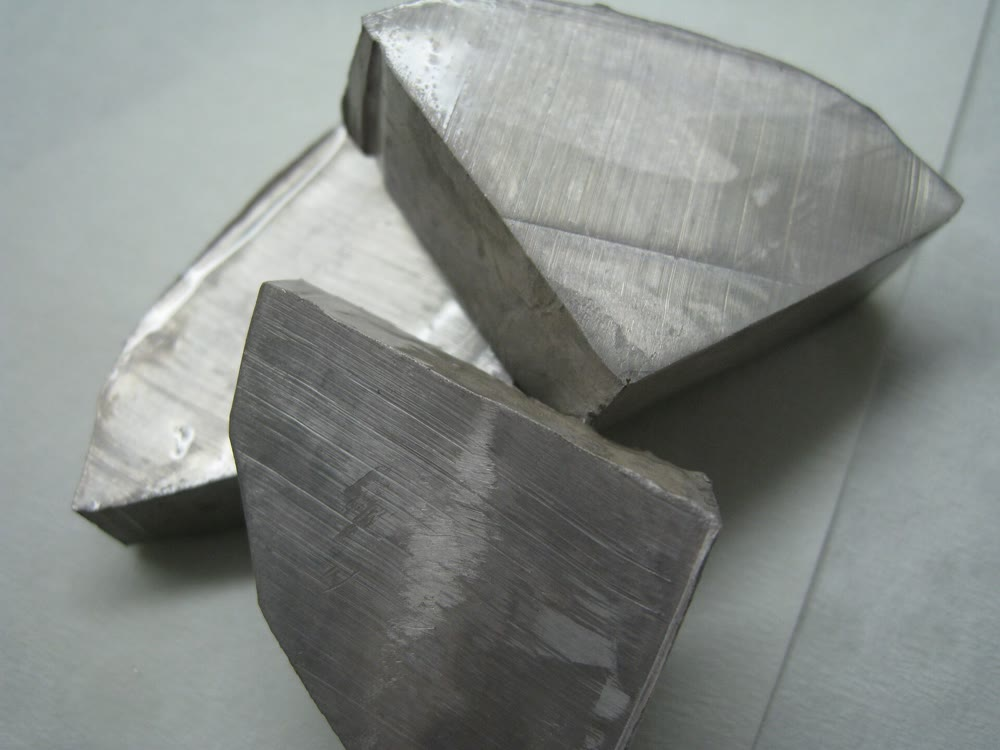
\includegraphics[width=\linewidth,height=4.4cm,keepaspectratio]{images/book1/sodium.jpg}

{\small O sódio, um \omterm{def:g10:electron-shells:family}{metal alcalino}, cortado com uma faca: mole e
prateado quando recém-cortado, ele escurece na hora ao \omterm{def:g4:air-a-mixture-of-gases:air}{ar}. Foto: Dnn87,
CC BY-SA 3.0.}
\end{minipage}\hfill
\begin{minipage}[b]{0.48\linewidth}\centering
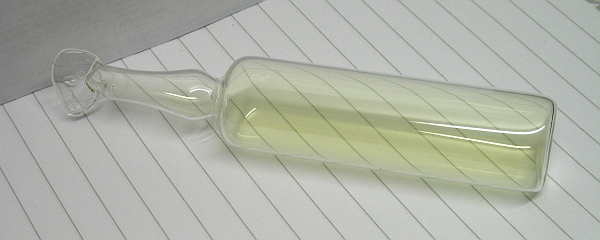
\includegraphics[width=\linewidth,height=4.4cm,keepaspectratio]{images/book1/chlorine-ampoule.jpg}

{\small O cloro, um \omterm{def:g10:electron-shells:family}{halogênio}: um gás amarelo-esverdeado, aqui lacrado
numa ampola de vidro. Foto: W.~Oelen, CC BY-SA 3.0.}
\end{minipage}
\end{omfigure}

\begin{inthelab}[O sódio na água]
Atrás de uma tela, o professor joga um pedaço de sódio do tamanho de um
grão de arroz numa bacia grande com água. Ele flutua, derrete numa
bolinha brilhante e dispara de um lado para o outro, chiando, até sumir;
o gás liberado é o hidrogênio, e a água que fica é básica.
\end{inthelab}

\begin{safety}{\ghs[0.75cm]{GHS02}\ghs[0.75cm]{GHS05}\quad\ghs[0.75cm]{GHS03}\ghs[0.75cm]{GHS06}}
% ledger: ghs:Na, ghs:Cl2
Sódio: libera hidrogênio inflamável com a água (GHS02), provoca
queimaduras graves (GHS05). Cloro: um gás oxidante (GHS03), tóxico se
inalado (GHS06), também irritante e muito tóxico para os organismos
aquáticos. Os dois só são manuseados pelo professor.
\end{safety}

\section{Os íons estáveis e a regra dos gases nobres}

\begin{definition}[Regras do dueto e do octeto]\label{def:g10:electron-shells:octet}
Os \omterm{def:g10:electron-shells:family}{gases nobres}, com uma \omterm{def:g10:electron-shells:configuration}{camada} externa completa, quase não reagem: a
configuração deles é especialmente estável. Quando os \omterm{def:g7:atoms-and-molecules:atom}{átomos} dos
primeiros elementos formam \omterm{def:g9:ions:ion}{íons}, eles ganham ou perdem \omterm{def:g9:inside-the-atom:nucleus}{elétrons} de modo
a alcançar a configuração do \omterm{def:g10:electron-shells:family}{gás nobre} mais próximo: dois \omterm{def:g9:inside-the-atom:nucleus}{elétrons} na
\omterm{def:g10:electron-shells:configuration}{camada} 1, como o hélio, para os \omterm{def:g7:atoms-and-molecules:atom}{átomos} mais leves --- a \emph{regra do
dueto}\index{regra do dueto} --- e oito \omterm{def:g9:inside-the-atom:nucleus}{elétrons} na \omterm{def:g10:electron-shells:configuration}{camada} externa, como
o neônio ou o argônio, para os outros --- a \emph{regra do
octeto}\index{regra do octeto}.
\end{definition}

\begin{example}[Íons previstos pela regra]\label{ex:g10:electron-shells:ions}
O sódio, $2.8.1$, perde o seu único \omterm{def:g10:electron-shells:valence}{elétron de valência}: \ce{Na+}, $2.8$,
como o neônio. O magnésio, $2.8.2$, perde dois: \ce{Mg^{2+}}. O alumínio,
$2.8.3$, perde três: \ce{Al^{3+}}. O cloro, $2.8.7$, ganha um: \ce{Cl-},
$2.8.8$, como o argônio. O oxigênio, $2.6$, ganha dois: \ce{O^{2-}}. O
enxofre, $2.8.6$: \ce{S^{2-}}. O lítio, $2.1$, perde um e fica com $2$,
como o hélio: \ce{Li+}.
\end{example}

\begin{omfigure}
\begin{tikzpicture}[font=\small]
  \foreach \x/\nm/\cfg/\col in {0/{Na}/{$1\mathrm{s}^2\,2\mathrm{s}^2\,2\mathrm{p}^6\,3\mathrm{s}^1$}/omDef,
      5.8/{\ce{Na+}}/{$1\mathrm{s}^2\,2\mathrm{s}^2\,2\mathrm{p}^6$}/omProp,
      11.0/{Ne}/{$1\mathrm{s}^2\,2\mathrm{s}^2\,2\mathrm{p}^6$}/gray} {
    \node[draw=\col, fill=\col!6, rounded corners=2pt, align=center, text width=3.4cm]
      at (\x,0) {\textbf{\nm}\\ \cfg};
  }
  \draw[->, thick, omProp] (2.0,0) -- (3.8,0) node[midway, above, font=\footnotesize] {perde 1 \ce{e-}};
  \node at (8.4,0) {$=$};
  \node[font=\footnotesize, align=center] at (8.4,-0.75) {mesma\\ configuração};
\end{tikzpicture}

{\small O \omterm{def:g9:ions:ion}{íon} sódio tem a configuração do neônio, o \omterm{def:g10:electron-shells:family}{gás nobre} mais
próximo.}
\end{omfigure}

\begin{remark}[Limites da regra]\label{rem:g10:electron-shells:limits}
A regra funciona bem para os vinte primeiros elementos e os seus \omterm{def:g9:ions:ion}{íons}
simples. Muitos elementos, como o ferro (\ce{Fe^{2+}} e \ce{Fe^{3+}}),
não a seguem; as razões, e uma descrição melhor dos \omterm{def:g9:inside-the-atom:nucleus}{elétrons}, são dadas
no volume do primeiro ano da universidade.
\end{remark}

\section{Exercícios}

\begin{exercise}[$\star$]\label{exo:g10:electron-shells:1}
Escreva as \omterm{def:g10:electron-shells:configuration}{configurações eletrônicas} do carbono ($Z = 6$), do nitrogênio
($Z = 7$) e do magnésio ($Z = 12$).
\end{exercise}

\begin{exercise}[$\star$]\label{exo:g10:electron-shells:2}
Quantos \omterm{def:g10:electron-shells:valence}{elétrons de valência} têm o carbono, o nitrogênio e o magnésio?
\end{exercise}

\begin{exercise}[$\star$]\label{exo:g10:electron-shells:3}
Em que período e em que grupo está o elemento de configuração
$1\mathrm{s}^2\,2\mathrm{s}^2\,2\mathrm{p}^6\,3\mathrm{s}^2\,3\mathrm{p}^3$?
\end{exercise}

\begin{exercise}[$\star$]\label{exo:g10:electron-shells:4}
Dê o nome das três famílias deste capítulo e dois elementos de cada uma.
\end{exercise}

\begin{exercise}[$\star$]\label{exo:g10:electron-shells:5}
Enuncie a \omterm{def:g10:electron-shells:octet}{regra do octeto}.
\end{exercise}

\begin{exercise}[$\star\star$]\label{exo:g10:electron-shells:6}
Usando a regra dos \omterm{def:g10:electron-shells:family}{gases nobres}, dê o \omterm{def:g9:ions:ion}{íon} formado pelo potássio
($Z = 19$) e pelo flúor ($Z = 9$), com as suas configurações.
\end{exercise}

\begin{exercise}[$\star\star$]\label{exo:g10:electron-shells:7}
Um elemento tem 2 \omterm{def:g9:inside-the-atom:nucleus}{elétrons} na terceira camada, e a terceira camada é a
sua \omterm{def:g10:electron-shells:configuration}{camada} externa. Dê a sua configuração, o seu \omterm{def:g9:inside-the-atom:atomic-number}{número atômico} e o seu
nome.
\end{exercise}

\begin{exercise}[$\star\star$]\label{exo:g10:electron-shells:8}
Usando os \omterm{def:g9:ions:ion}{íons} estáveis, escreva a fórmula do \omterm{def:g9:ions:ionic-compound}{composto iônico} formado
pelo magnésio e pelo cloro, e depois pelo alumínio e pelo oxigênio.
\end{exercise}

\begin{exercise}[$\star\star$]\label{exo:g10:electron-shells:9}
Olhe a tabela dos vinte primeiros elementos. Que elementos têm o mesmo
número de \omterm{def:g10:electron-shells:valence}{elétrons de valência} que o oxigênio?
\end{exercise}

\begin{exercise}[$\star\star$]\label{exo:g10:electron-shells:10}
Por que o neônio, ao contrário do sódio e do cloro, não forma \omterm{def:g9:ions:ion}{íons} nas
\omterm{def:g7:chemical-reactions:reaction}{reações químicas}?
\end{exercise}

\begin{exercise}[$\star\star$]\label{exo:g10:electron-shells:11}
O \omterm{def:g9:ions:ion}{íon} \ce{X^{2+}} tem a configuração do argônio. Encontre $X$.
\end{exercise}

\begin{exercise}[$\star\star\star$]\label{exo:g10:electron-shells:12}
O hélio tem 2 \omterm{def:g10:electron-shells:valence}{elétrons de valência}, mas fica no \omterm{def:g9:periodic-table-first-look:period}{grupo} 18, e não no
\omterm{def:g9:periodic-table-first-look:period}{grupo} 2. Explique usando a sua configuração.
\end{exercise}

\begin{exercise}[$\star\star\star$]\label{exo:g10:electron-shells:13}
O potássio reage com a água de modo ainda mais violento que o sódio.
Usando a distância do \omterm{def:g10:electron-shells:valence}{elétron de valência} ao \omterm{def:g9:inside-the-atom:nucleus}{núcleo}, sugira por quê.
\end{exercise}

\begin{exercise}[$\star\star\star$]\label{exo:g10:electron-shells:14}
Dê as configurações de \ce{S^{2-}}, \ce{Cl-}, \ce{K+} e \ce{Ca^{2+}}.
O que elas têm em comum?
\end{exercise}

\begin{exercise}[$\star\star\star$]\label{exo:g10:electron-shells:15}
Um elemento do período 3 forma o \omterm{def:g9:ions:ion}{íon} \ce{Y^{3-}}. Encontre o seu grupo,
a sua configuração e o seu nome.
\end{exercise}

\section{Problema: rubi, safira e coríndon}

\begin{problem}[{Problema de fim de semana --- os elétrons por trás de
uma pedra preciosa: de duas configurações ao número de elétrons
transferidos num grama}]
\label{pb:g10:electron-shells:1}
Os rubis e as safiras são formas preciosas do coríndon, um \omterm{def:g9:ions:ionic-compound}{composto
iônico} de alumínio e oxigênio; um traço de outros \omterm{def:g9:periodic-table-first-look:metal}{metais} dá a eles as
suas cores. O coríndon é duro o bastante para riscar quase tudo, e o
coríndon em pó é usado para polir lentes. Tome a massa de um \omterm{def:g9:inside-the-atom:proton}{núcleon}
como \qty{1.67e-27}{kg}; o alumínio-27 tem 27 \omterm{def:g9:inside-the-atom:proton}{núcleons}, o oxigênio-16
tem 16.

\medskip
\noindent\textbf{Parte I --- Os \omterm{def:g7:atoms-and-molecules:atom}{átomos}.}
\begin{enumerate}
  \item Dê os números de \omterm{def:g9:inside-the-atom:proton}{prótons} e de \omterm{def:g9:inside-the-atom:nucleus}{elétrons} de um \omterm{def:g7:atoms-and-molecules:atom}{átomo} de alumínio
        ($Z = 13$) e de um \omterm{def:g7:atoms-and-molecules:atom}{átomo} de oxigênio ($Z = 8$).
  \item Escreva as suas \omterm{def:g10:electron-shells:configuration}{configurações eletrônicas}.
  \item Quantos \omterm{def:g10:electron-shells:valence}{elétrons de valência} tem cada um? Em que período e em
        que grupo está cada um?
  \item O alumínio é um \omterm{def:g9:periodic-table-first-look:metal}{metal} ou um \omterm{def:g9:periodic-table-first-look:metal}{não metal}? E o oxigênio?
\end{enumerate}

\medskip
\noindent\textbf{Parte II --- Os \omterm{def:g9:ions:ion}{íons}.}
\begin{enumerate}[resume]
  \item Usando a \omterm{def:g10:electron-shells:octet}{regra do octeto}, que \omterm{def:g9:ions:ion}{íon} o alumínio forma? Escreva a
        sua configuração.
  \item Que \omterm{def:g9:ions:ion}{íon} o oxigênio forma? Escreva a sua configuração.
  \item Que \omterm{def:g10:electron-shells:family}{gás nobre} tem a mesma configuração que os dois \omterm{def:g9:ions:ion}{íons}?
  \item Quantos \omterm{def:g9:inside-the-atom:nucleus}{elétrons} um \omterm{def:g7:atoms-and-molecules:atom}{átomo} de alumínio perde, e quantos um \omterm{def:g7:atoms-and-molecules:atom}{átomo}
        de oxigênio ganha?
\end{enumerate}

\medskip
\noindent\textbf{Parte III --- A fórmula.}
\begin{enumerate}[resume]
  \item Encontre a fórmula do coríndon, o composto neutro desses \omterm{def:g9:ions:ion}{íons}.
  \item Numa unidade de fórmula, quantos \omterm{def:g9:inside-the-atom:nucleus}{elétrons} são perdidos pelos
        \omterm{def:g7:atoms-and-molecules:atom}{átomos} de alumínio? E ganhos pelos \omterm{def:g7:atoms-and-molecules:atom}{átomos} de oxigênio?
  \item Por que esses dois números têm de ser iguais?
  \item Um rubi contém um traço de \omterm{def:g9:ions:ion}{íons} cromo \ce{Cr^{3+}} no lugar de
        alguns \ce{Al^{3+}}. Por que um \omterm{def:g9:ions:ion}{íon} \ce{Cr^{3+}} pode tomar o
        lugar de um \omterm{def:g9:ions:ion}{íon} \ce{Al^{3+}} sem desequilibrar as cargas?
\end{enumerate}

\medskip
\noindent\textbf{Parte IV --- Um grama de coríndon.}
\begin{enumerate}[resume]
  \item Quantos \omterm{def:g9:inside-the-atom:proton}{núcleons} há numa unidade de fórmula de coríndon?
  \item Calcule a massa de uma unidade de fórmula (desprezando os
        \omterm{def:g9:inside-the-atom:nucleus}{elétrons}).
  \item Quantas unidades de fórmula há em \qty{1}{g} de coríndon?
  \item Quantos \omterm{def:g9:ions:ion}{íons} \ce{Al^{3+}} e quantos \omterm{def:g9:ions:ion}{íons} \ce{O^{2-}} isso
        representa?
  \item Por que os \omterm{def:g9:inside-the-atom:nucleus}{elétrons} podem ser desprezados na questão 14?
  \item Quantos \omterm{def:g9:inside-the-atom:nucleus}{elétrons} foram transferidos do alumínio para o oxigênio
        para formar \qty{1}{g} de coríndon?
\end{enumerate}
\end{problem}
